\pagebreak
\subsection{Latlon coordinates NetCDF GRID\_GEOMETRY\_ECCO}
\newp
\begin{longtable}{|p{0.1\textwidth}|p{0.5\textwidth}|}
\caption{Variables in the dataset GRID\_GEOMETRY\_ECCO}
\label{tab:table-GRID_GEOMETRY_ECCO-fields} \\ 
\hline \endhead \hline \endfoot
\rowcolor{lightgray} \textbf{Dataset:} & \textbf{GRID\_GEOMETRY\_ECCO} \\ \hline
Field: &hFacC \\ \hline
Field: &maskC \\ \hline
\end{longtable}

\pagebreak
\subsubsection{Latlon coordinates Variable hFacC}
\begin{longtable}{|m{0.06\textwidth}|m{0.41\textwidth}|m{0.39\textwidth}|m{0.06\textwidth}|}
\caption{CDL description of GRID\_GEOMETRY\_ECCO's hFacC variable}
\label{tab:table-GRID_GEOMETRY_ECCO_hFacC} \\ 
\hline \endhead \hline \endfoot
\rowcolor{lightgray} \textbf{Storage Type} & \textbf{Variable Name} & \textbf{Description} & \textbf{Unit} \\ \hline
float64 & hFacC & vertical open fraction of grid cell & 1 \\ \hline
\rowcolor{lightgray}  \multicolumn{4}{|p{1.00\textwidth}|}{\textbf{CDL Description}} \\ \hline
\multicolumn{4}{|p{1.00\textwidth}|}{\makecell{\parbox{1\textwidth}{float64 hFacC(Z, latitude, longitude)\\
\hspace*{0.5cm}hFacC: \_FillValue = 9.969209968386869e+36\\
\hspace*{0.5cm}hFacC: coverage\_content\_type = modelResult\\
\hspace*{0.5cm}hFacC: long\_name = vertical open fraction of grid cell\\
\hspace*{0.5cm}hFacC: units = 1}}} \\ \hline
\rowcolor{lightgray} \multicolumn{4}{|p{1.00\textwidth}|}{\textbf{Comments}} \\ \hline
\multicolumn{4}{|p{1\textwidth}|}{Grid cells may be fractionally closed in the vertical. The open vertical fraction is hFacC. The model allows for partially-filled cells to represent topographic variations more smoothly (hFacC < 1). Completely closed (dry) tracer grid cells have hFacC = 0. Note: the lat-lon gridded hFacC is spatially-averaged from the hFacC field on the lat-lon-cap (llc90) model native grid. The total ocean volume of the ECCO V4r4 lat-lon gridded fields is within 0.05\% of the total ocean volume of the native grid fields.} \\ \hline
\end{longtable}

\begin{figure}[H]
\centering
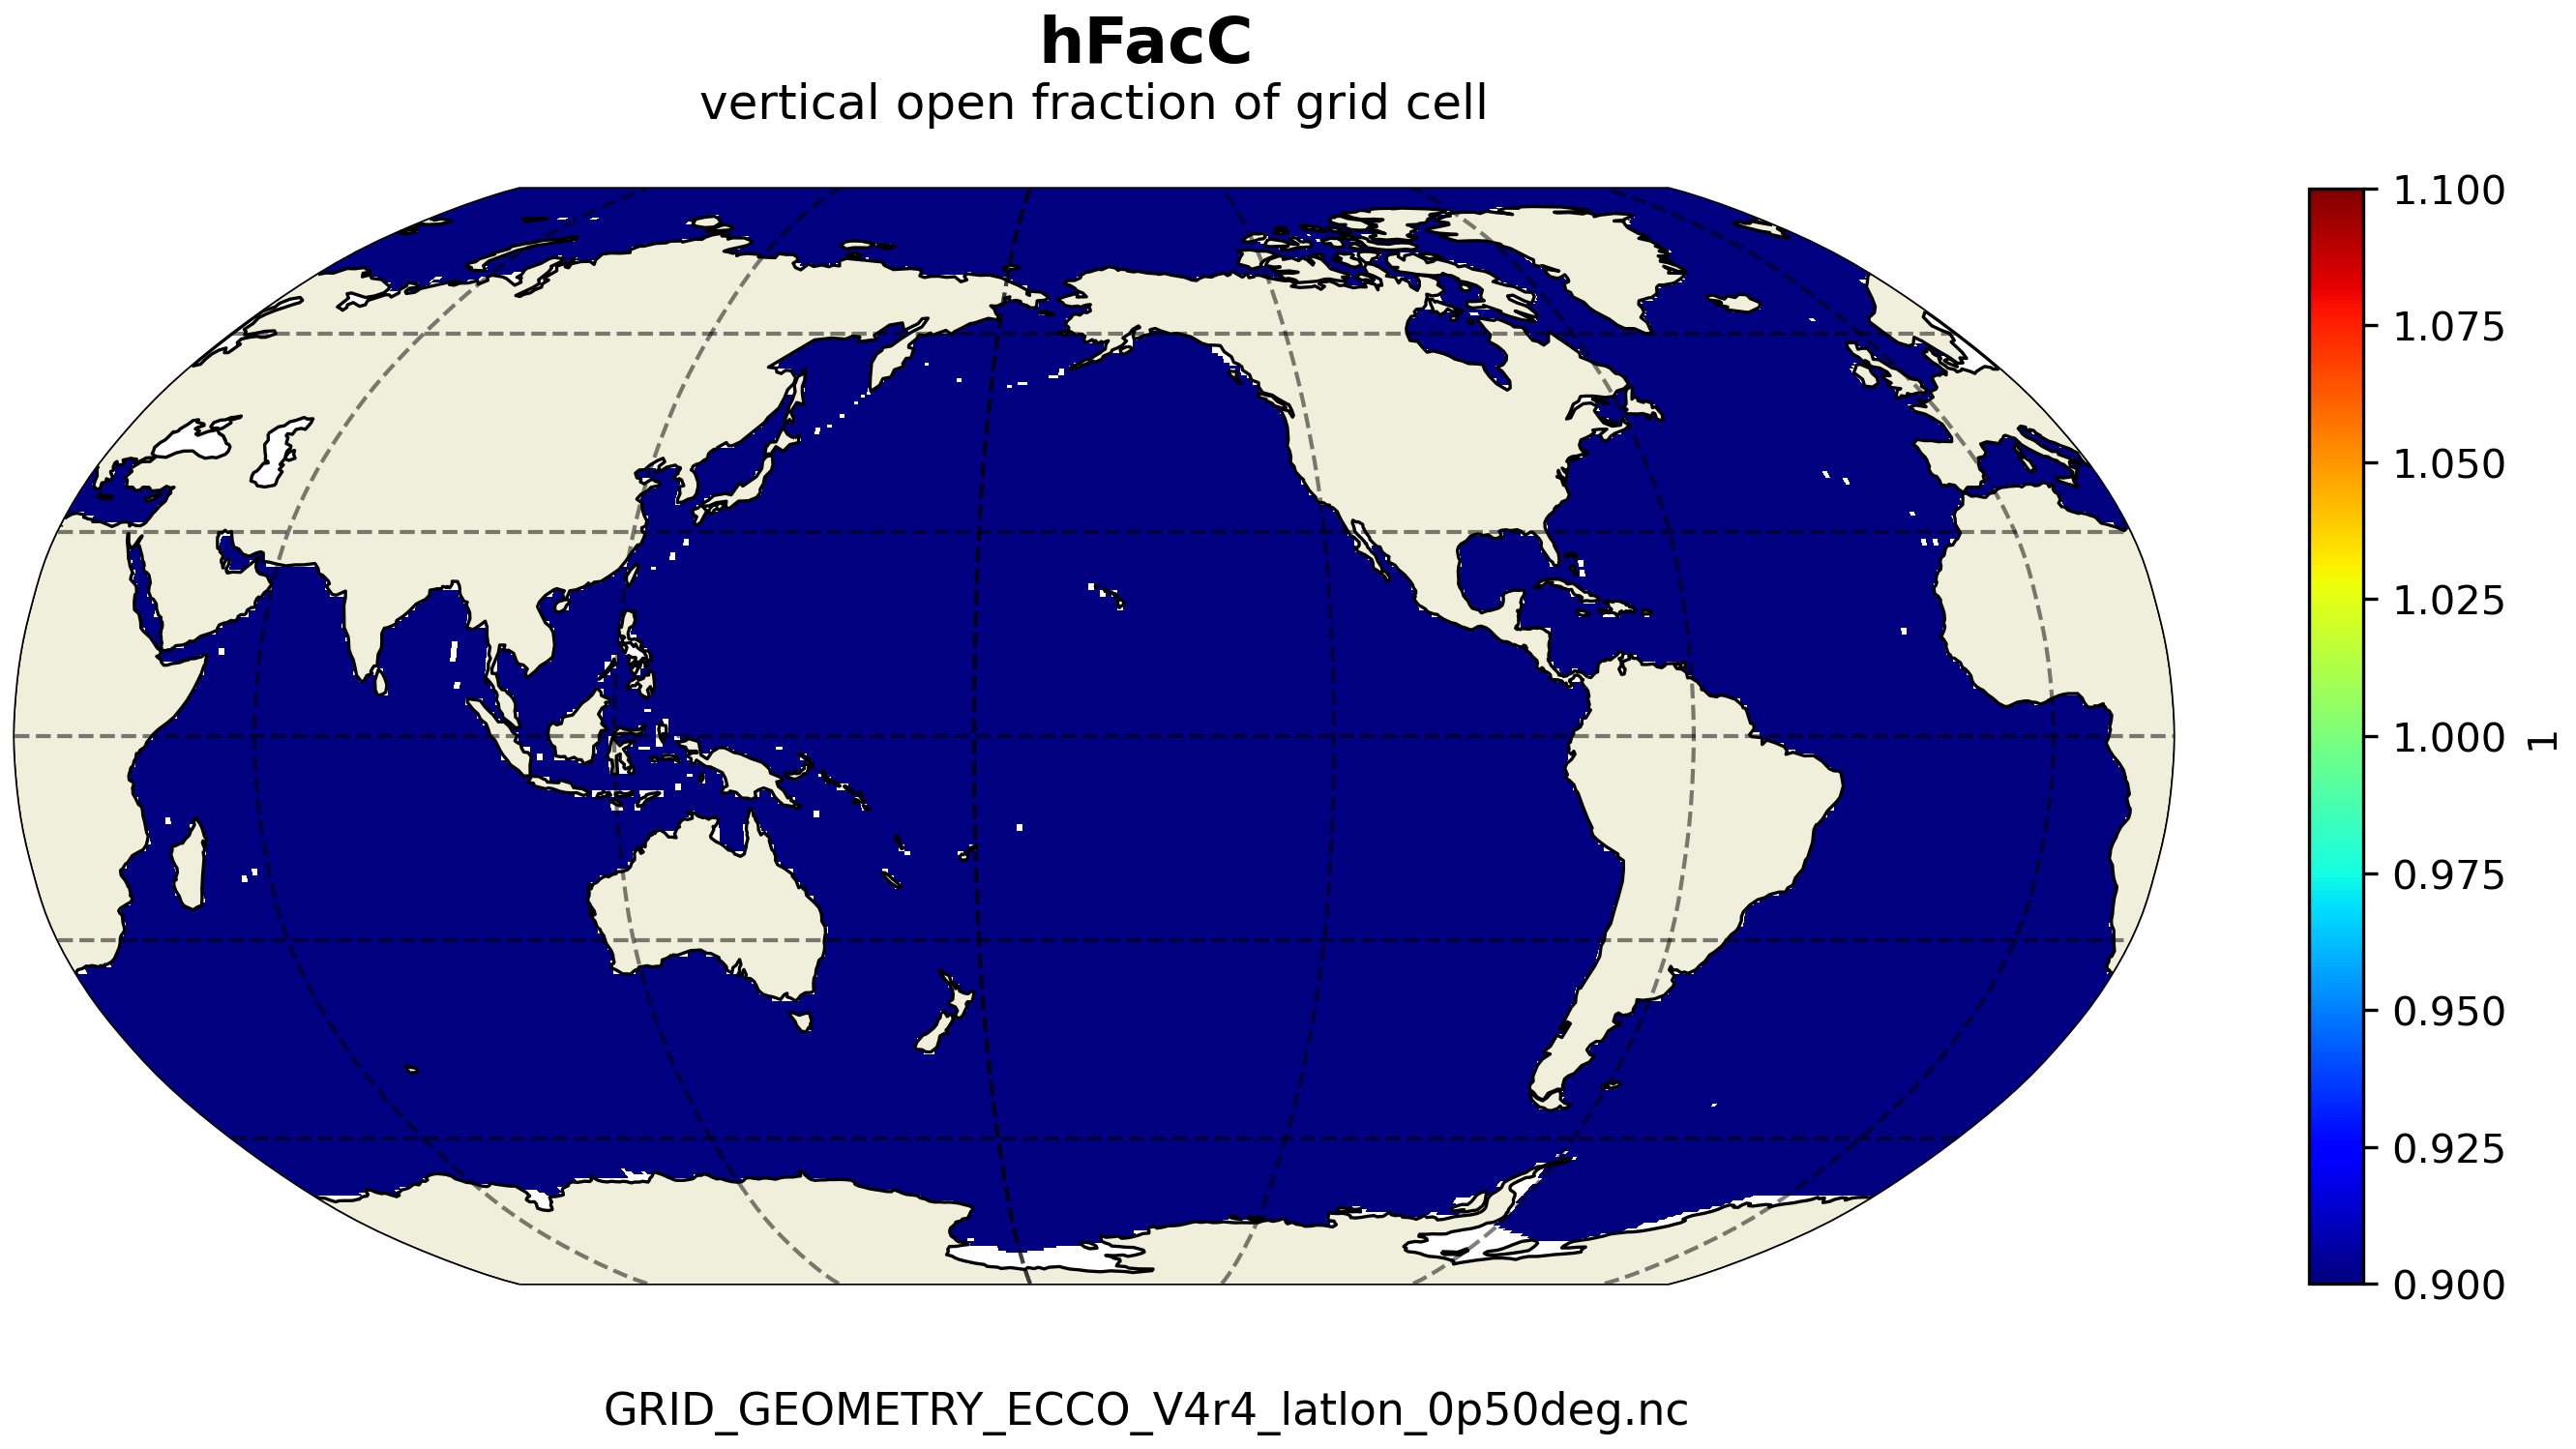
\includegraphics[scale=0.55]{../images/plots/latlon_plots_coords/Geometry_Parameters_for_the_0.5_degree_Lat-Lon_Model_Grid_(Version_4_Release_4)/hFacC.png}
\caption{Dataset: GRID\_GEOMETRY\_ECCO Variable: hFacC}
\label{tab:table-GRID_GEOMETRY_ECCO_hFacC-Plot}
\end{figure}
\pagebreak
\subsubsection{Latlon coordinates Variable maskC}
\begin{longtable}{|m{0.06\textwidth}|m{0.41\textwidth}|m{0.39\textwidth}|m{0.06\textwidth}|}
\caption{CDL description of GRID\_GEOMETRY\_ECCO's maskC variable}
\label{tab:table-GRID_GEOMETRY_ECCO_maskC} \\ 
\hline \endhead \hline \endfoot
\rowcolor{lightgray} \textbf{Storage Type} & \textbf{Variable Name} & \textbf{Description} & \textbf{Unit} \\ \hline
bool & maskC & wet/dry boolean mask for grid cell & N/A \\ \hline
\rowcolor{lightgray}  \multicolumn{4}{|p{1.00\textwidth}|}{\textbf{CDL Description}} \\ \hline
\multicolumn{4}{|p{1.00\textwidth}|}{\makecell{\parbox{1\textwidth}{bool maskC(Z, latitude, longitude)\\
\hspace*{0.5cm}maskC: \_FillValue = 1\\
\hspace*{0.5cm}maskC: coverage\_content\_type = modelResult\\
\hspace*{0.5cm}maskC: long\_name = wet/dry boolean mask for grid cell}}} \\ \hline
\rowcolor{lightgray} \multicolumn{4}{|p{1.00\textwidth}|}{\textbf{Comments}} \\ \hline
\multicolumn{4}{|p{1\textwidth}|}{True for grid cells with nonzero open vertical fraction (hFacC > 0), otherwise False.} \\ \hline
\end{longtable}

\begin{figure}[H]
\centering
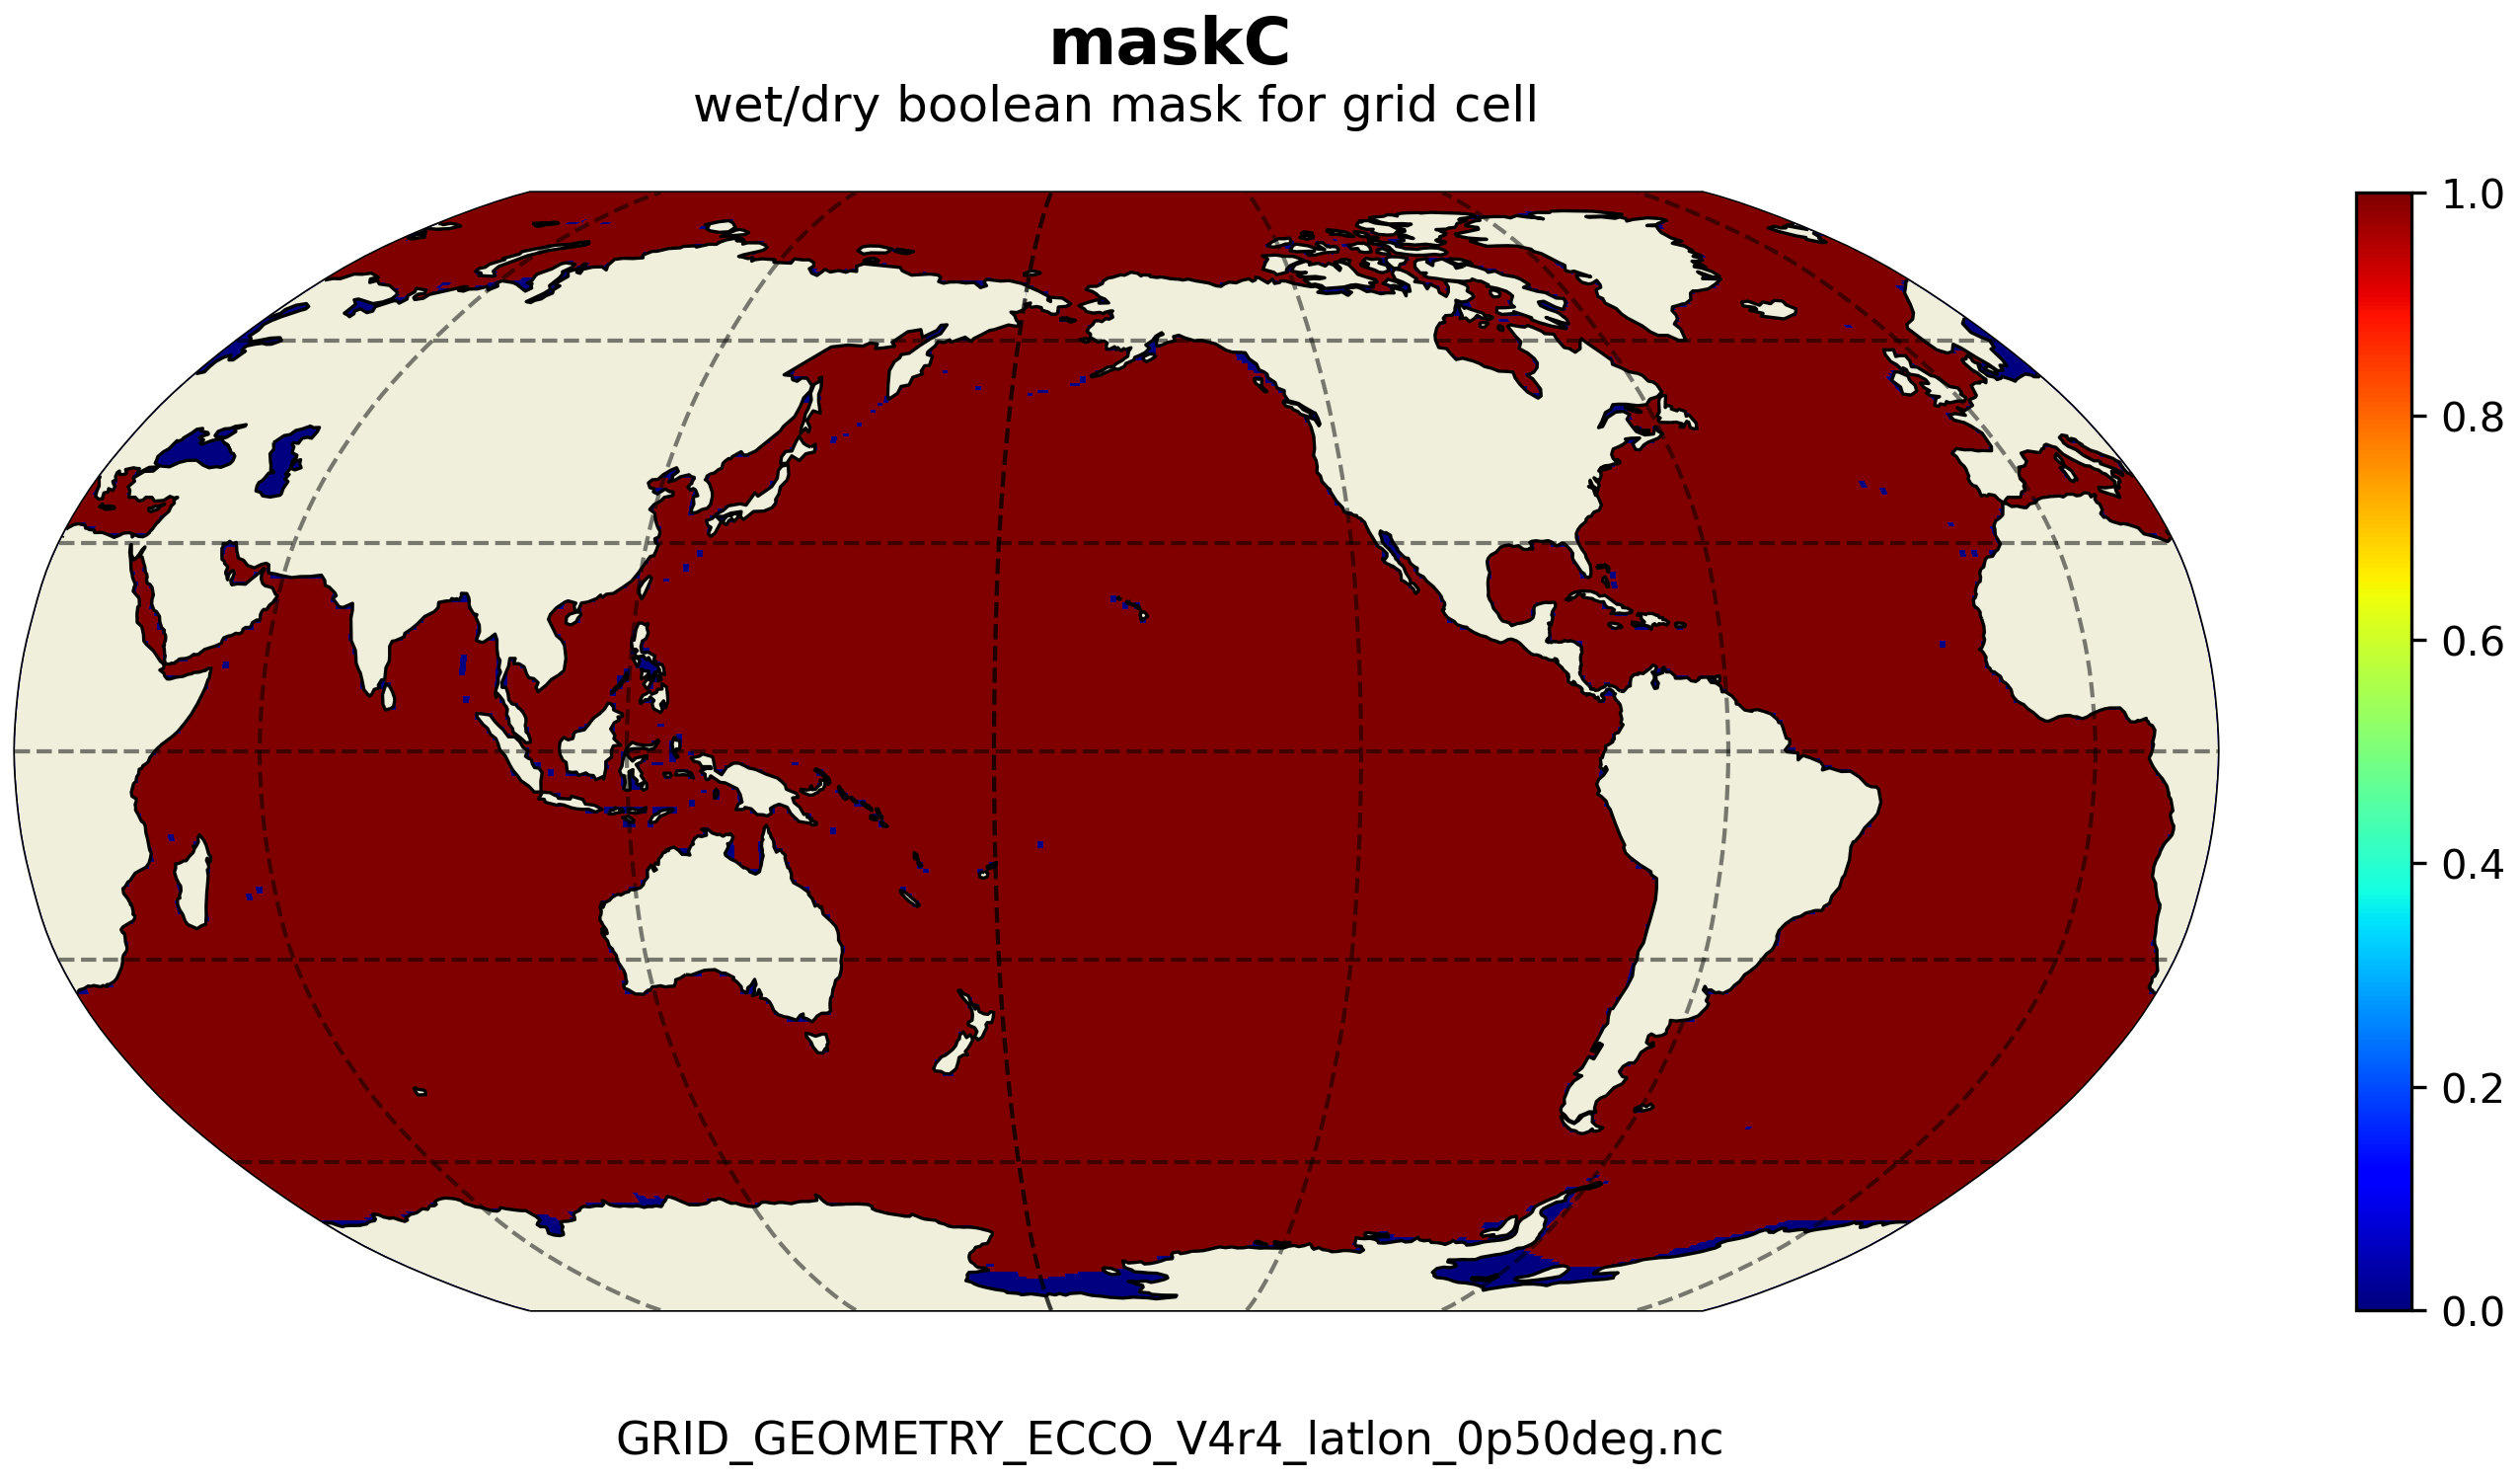
\includegraphics[scale=0.55]{../images/plots/latlon_plots_coords/Geometry_Parameters_for_the_0.5_degree_Lat-Lon_Model_Grid_(Version_4_Release_4)/maskC.png}
\caption{Dataset: GRID\_GEOMETRY\_ECCO Variable: maskC}
\label{tab:table-GRID_GEOMETRY_ECCO_maskC-Plot}
\end{figure}